\section{Esercitazione 1}

\subsection{Librerie di base per il calcolo seriale in Algebra Lineare Numerica (BLAS)}

Gran parte dei problemi del calcolo scientifico ed ingegneristico richiede di risolvere uno o più problemi dell'algebra lineare numerica (ALN):

\begin{itemize}

	\item Risoluzione di sistemi lineari;
	\item Risoluzione di problemi ai minimi quadrati;
	\item Ricerca di autovalori e/o autovettori;
	\item Calcolo della SVD (valori e vettori singolari);

\end{itemize}

Inoltre, la risoluzione di questi problemi è generalmente una percentuale considerevole del costo computazionale totale richiesto per la risoluzione del problema globale; questo costo si traduce spesso in ore o giorni di tempo-macchina impiegato. Dunque, implementare in modo efficiente gli algoritmi che risolvono i problemi dell'algebra lineare numerica è estremamente importante dal punto di vista applicativo ed è anche per questo che trattiamo questo caso più approfonditamente.
Un secondo motivo è dovuto al fatto che esistono in rete delle librerie che rappresentano lo stato dell'arte per questi problemi e sono molto ben costruite anche dal punto di vista della implementazione e distribuzione del software numerico: BLAS, LAPACKe ATLAS (disponibili al sito www.netlib.org/blas , /lapack e /atlas).

Gli algoritmi di algebra lineare numerica hanno in comune un insieme relativamente piccolo e stabile di operazioni di base, che svolge la quasi totalità dei calcoli necessari negli algoritmi di ALN. Questo fatto giustifica lo sforzo di creazione di una libreria che implementi queste funzione di base. La libreria BLAS è organizzata in tre livelli:
operazioni che lavorano su vettori e producono uno scalare  (es. il prodotto interno, o scalare, tra due vettori colonna: v' * w), operazioni tra vettori e matrici o che comunque producono una matrice (es. il prodotto esterno tra due vettori colonna: v * w'), operazioni tra matrici (es. il prodotto di due matrici).

Un vantaggio rilevante di aver creato la BLAS è che questa può essere ottimizzata per ogni singola macchina ed in questo modo gli algoritmi di ALN possono diventare ``portabili'' anche dal punto di vista delle prestazioni di calcolo e non solo da quello della sintassi, semplicemente chiamando le routines della BLAS ove possibile.

Ora, ha senso chiedersi se le operazioni di livello 1, 2 o 3 raggiungono le stesse prestazioni di calcolo. Lo vediamo implementando lo stesso identico algoritmo, il prodotto di due matrici C = A * B, in tre modi diversi, corrispondenti all'utilizzo esclusivo di operazioni di livello 1, di livello 2 e di livello 3.

\begin{figure}[ht!]
\centering
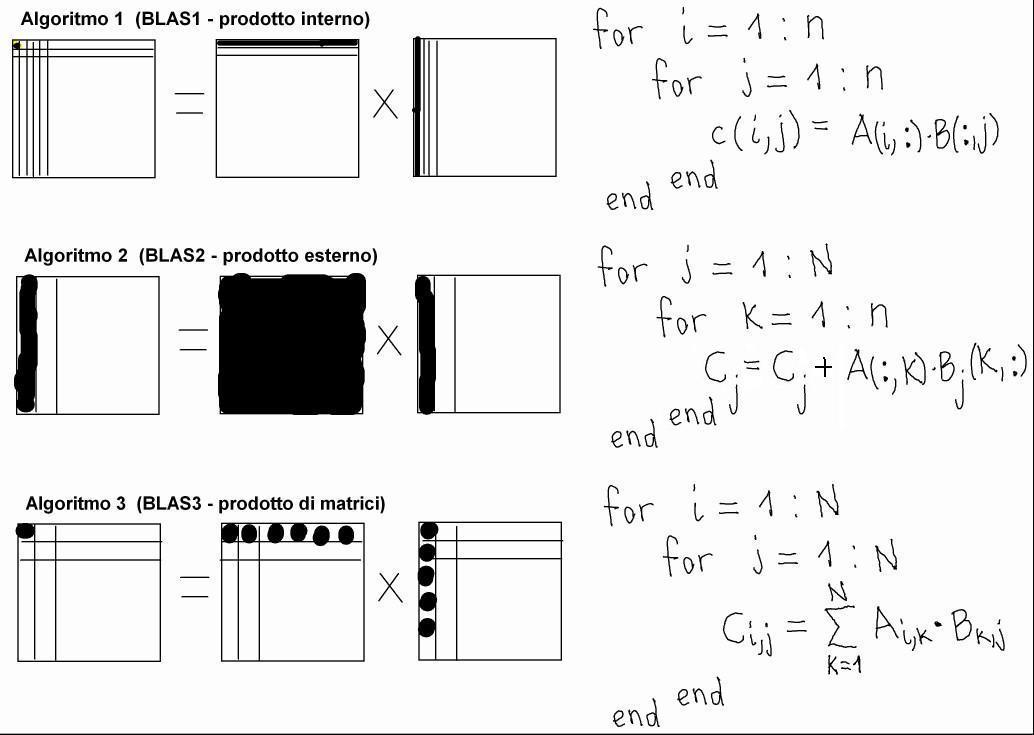
\includegraphics[width=130mm]{images/implementazioni_prodotto_di_matrici.jpg}
\caption{Algoritmi BLAS}
\label{overflow}
\end{figure}

Se facciamo eseguire questi algoritmi da un calcolatore per il quale la libreria BLAS è stata ottimizzata, otteniamo risultati di questo tipo:

\begin{figure}[ht!]
\centering
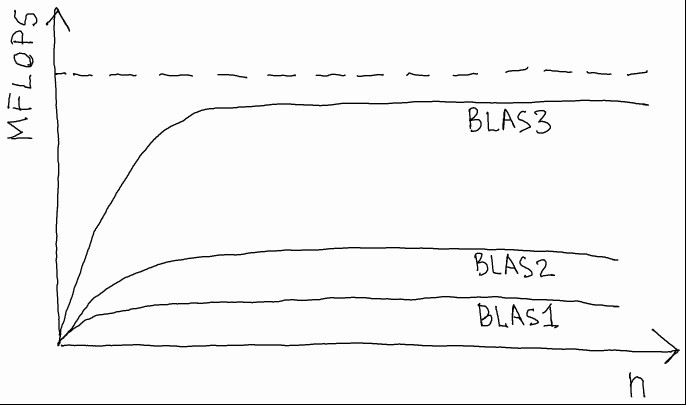
\includegraphics[width=130mm]{images/prestazioni_BLAS.JPG}
\caption{Prestazioni BLAS}
\label{overflow}
\end{figure}

e dunque, formulazioni identiche dal punto di vista matematico possono portare a performance molto differenti dal punto di vista delle prestazioni di calcolo. Notare che, in questo esempio, il numero di operazioni in virgola mobile è sempre uguale a $2*n^3$ in tutti e tre i casi.

Questo risultato ha validità generale: le operazioni BLAS3 sono molto più veloci delle BLAS2 e BLAS1 nelle macchine di calcolo di ultima generazione, e dunque vanno utilizzate il più possibile negli algoritmi di ALN per avere buone prestazioni dal calcolatore.

\subsection{Calcolo delle prestazioni ottenibili dalle BLAS}

Vediamo di spiegare perchè le routines BLAS3 sono più performanti ed in quali condizioni. Una caratteristica sempre più frequente dei problemi di ALN che sorgono nelle applicazioni reali è quella di avere matrici di grandi dimensioni, e dunque una criticità nasce dal punto di vista dell'occupazione di memoria.
Vediamo uno schema dell'organizzazione gerarchica della memoria nei calcolatori attuali $(d_s, d_p e d_c$ indicano il tempo necessario al trasferimento di un'unità di dati):

\begin{figure}[ht!]
\centering
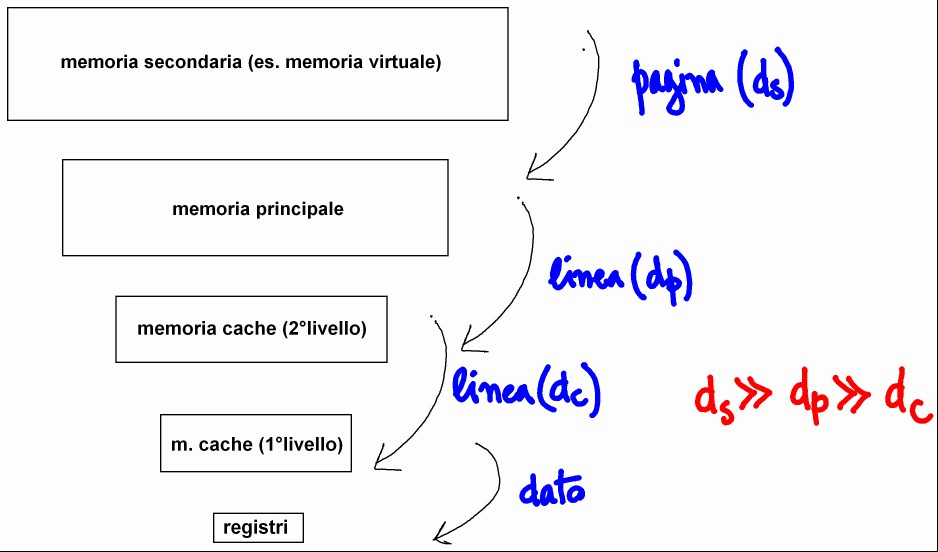
\includegraphics[width=130mm]{images/organizzazione_memorie.JPG}
\caption{Organizzazione memorie}
\label{overflow}
\end{figure}

Lo sviluppo tecnologico delle CPU moderne ha portato a richiedere tempi ridottissimi per l'esecuzione di un'operazione in virgola mobile; non così è stato per la velocità di trasferimento dei dati tra i livelli di memoria: dato che per eseguire un'operazione in virgola mobile la CPU deve poter caricare gli operandi dalla memoria veloce (cache) nei suoi registri e che questa, per ragioni tecnologiche e di costo, ha dimensioni limitate, la criticità maggiore per le prestazioni sul tempo di calcolo è mantenere impegnata la CPU.
In piccola parte il microprocessore ed il compilatore hanno dei mezzi per mascherare i tempi di trasferimento dei dati, ma per ottenere un buon risultato è necessario che l'algoritmo di calcolo e la sua implementazione siano progettati in modo che:

\begin{center}

$Noperazioni f.p.  >>   Ntrasferimenti di dati$

\end{center}

Esiste una misura precisa ed un valore massimo di velocità raggiungibile dalle prestazioni di calcolo. La velocità massima di calcolo raggiungibile da una CPU dipende dalla frequenza di clock, dal numero di cicli di clock necessari ad eseguire un'operazione in virgola mobile (floating-point) e da quante unità hardware per il calcolo f.p. sono presenti. Quindi la velocità massima può essere calcolata dai dati di targa della macchina.
Se il programma prevede una sequenza (lunga) di operazioni in virgola mobile senza istruzioni di altro tipo e se il processore trova sempre disponibili gli operandi nella memoria veloce, il calcolo procede alla massima velocità possibile.

Supponiamo $m = mA + mB + mC$ , cioè scomposto nella somma degli accessi alla matrice A, alla matrice B ed alla matrice C  e calcoliamone il valore. Ispezionando l'implementazione dell'algoritmo, è possibile determinare il numero di accessi effettuati (vedere figura seguente):

\begin{figure}[ht!]
\centering
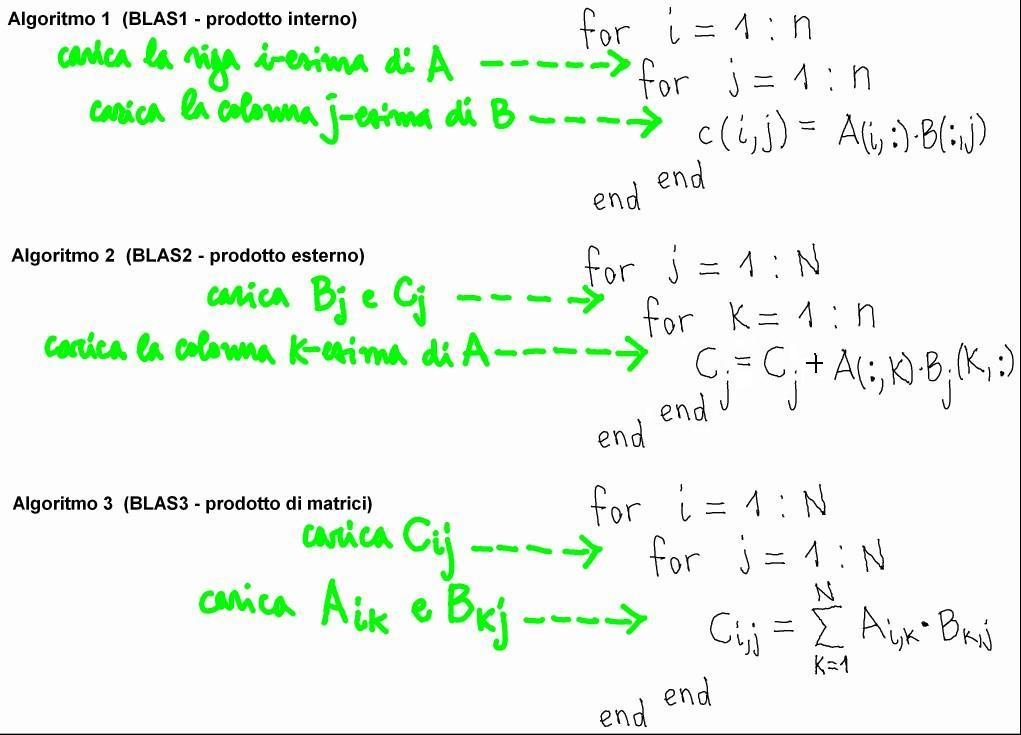
\includegraphics[width=130mm]{images/accessi_alla_memoria_per_prodotto_di_matrici.JPG}
\caption{Accessi alla memoria per prodotto di matrici}
\label{overflow}
\end{figure}

\subsection{Ottimizzazione empirica automatizzata della libreria software BLAS: il progetto ATLAS}

Recentemente è stato portato a termine un progetto molto interessante riguardo alle BLAS: la costruzione di un software che durante la sua esecuzione, genera la libreria BLAS ottimizzata per la macchina su cui è in esecuzione.
Questo software è disponibile gratuitamente al sito :   www.netlib.org/atlas    (attenzione: la sua esecuzione richiede in media due-tre ore su un PC, però funziona in modo completamente automatico e sicuro).
Il suo successo è notevole, dato che riesce ad ottenere ottimizzazioni delle librerie tali da raggiungere le prestazioni ottenute dalle librerie commerciali, ottimizzate ``a mano'' da esperti.
Provandolo su un PC e confrontandone le prestazioni con le BLAS ``generali'' scaricate da www.netlib.org/blas si può notare che che la versione ``atlas'' delle BLAS è decine di volte più veloce delle BLAS ``generali'', già per una moltiplicazione di matrici di dimensione 1000.
Questo dimostra come le prestazioni di calcolo possono essere ottenute solo sfruttando in maniera sapiente le risorse hardware a disposizione, che possono variare considerevolmente anche solo restando nel mondo del PC (es. un parametro fondamentale è la dimensione della memoria cache).

\subsection{Esercizi}

\subsubsection{Esercizio 1}

 Costruire un programma in linguaggio Matlab/Octave che esegua il calcolo del prodotto di due  matrici A e B di dimensione n x n, utilizzando la singola istruzione $C = A*B$, per i valori di n presi tra 10 e 2350 con passo=10,  calcoli il tempo di esecuzione di ogni prodotto e faccia il grafico ``$(n, tempo)$''. Commentare l'andamento del grafico.

NOTA: \textit{il tempo di esecuzione, su un PC con processore a 1.8GHz, risulta essere pari a 23 sec per l'ultima moltiplicazione (n=2350) e pari a 22 minuti per il programma complessivo; si consiglia di fare alcune prove con valori di ``n'' bassi ed eventualmente fermarsi ad n < 2350.}

\lstinputlisting[style=customat, caption=Esercizio 1]{../Esercitazione1/esercizio1.m}

\subsubsection{Esercizio 2}

Costruire un programma in linguaggio Matlab/Octave che, date due matrici A e B di dimensione $n x n$, nei casi $n = 200, 800, 3200, 4000, 4800$, calcoli il prodotto ``per componenti'' della prima riga di A e di B utilizzando una sola istruzione, ne calcoli il tempo di esecuzione $t_riga$, e poi faccia lo stesso con la prima colonna. 

Il programma deve poi creare un grafico ``$(n, t_col / t_riga)$''.  Spiegare con un breve commento perchè questa differenza nei tempi di esecuzione.  [suggerimento: l'estensione Numeric per Python è scritta in linguaggio C e quindi le matrici vengono memorizzate in un vettore in cui vengono inserite per righe.  Notare che in Matlab, come in FORTRAN, le matrici vengono memorizzate per colonne].

NOTA: \textit{il tempo di esecuzione, per n>=4000 potrebbe diventare sostanzialmente lungo: fare attenzione e, a quel punto, fermarsi}.

\lstinputlisting[style=customat, caption=Esercizio 1]{../Esercitazione1/esercizio2.m}

\subsubsection{Esercizio 3}

Costruire un programma in linguaggio Matlab/Octave che esegua il calcolo del prodotto di due  matrici A e B di dimensione n x n e calcoli i singoli tempi di esecuzione, utilizzando:

\begin{itemize}

	\item L'istruzione Matlab/Octave C=A*B;
	\item Un algoritmo scritto in Matlab/Octave che usi operazioni BLAS3 (vedi sopra), chiamando N3 il numero di blocchi quadrati in cui viene suddivisa la matrice;
	\item Un algoritmo scritto in Matlab/Octave che usi operazioni BLAS2 (vedi sopra), chiamando N2 il numero di blocchi di colonne in cui viene suddivisa la matrice;
	\item Un algoritmo scritto in Matlab/Octave che usi operazioni BLAS1 (vedi sopra).

\end{itemize}

Provare il programma per un valore di n più elevato possibile e che sia una potenza di 2, diciamo $2^j$ (cominciare da $n = 2^9 = 512$ ) e per $N2,N3 = 2^k$ per $k=1,2,...,j$. 

Spiegare in qualche riga di commento le differenze nei tempi di esecuzione.

\lstinputlisting[style=customat, caption=Esercizio 1]{../Esercitazione1/esercizio3.m}